%Chapter 3

\renewcommand{\thechapter}{3}

\chapter{Apparatus}
\label{ch:apparatus}

\section{UMER Layout}

UMER is laid out as a 36-sided polygon, comprised of 18 modular $20^o$ sections. Each section houses 2 dipole magnets over $10^o$ pipe bends and 4 quadrupole magnets in a FODO (focusing-defocusing) arrangement.

\section{UMER Beams}
	\subsection{Generation and Detection of Low-Current Beam}
	
	%%%%%%%%%%%%%%%%%%%%%%%%%%%%%%%%%%%%%%%%%%%%%%%%%%%%%%%%%%%%%%%%%%%%%%%%%%%%%%%%%%%%%%%%%%%%%%%%%%%%%%%%%%%%%%%%%%%%%%%%
	% IPAC 2015
	%%%%%%%%%%%%%%%%%%%%%%%%%%%%%%%%%%%%%%%%%%%%%%%%%%%%%%%%%%%%%%%%%%%%%%%%%%%%%%%%%%%%%%%%%%%%%%%%%%%%%%%%%%%%%%%%%%%%%%%%
	\section{Negligible space charge beam}

\begin{figure}
\begin{center}
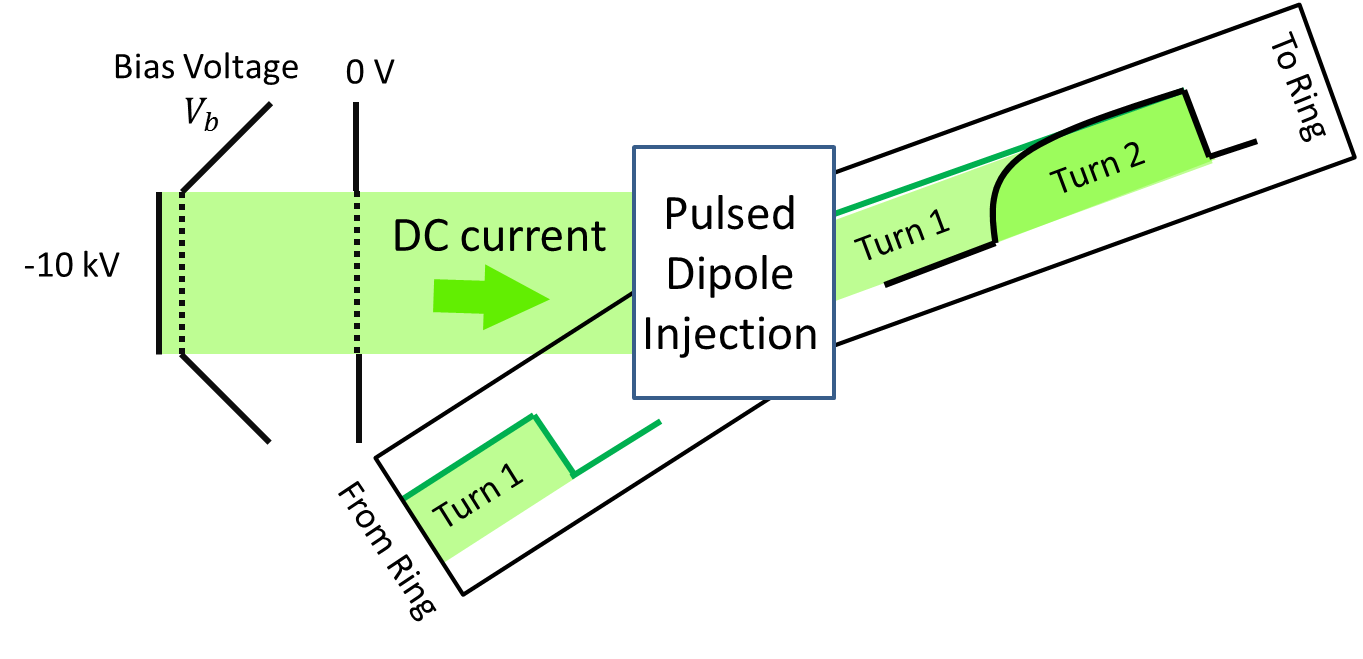
\includegraphics[width=\textwidth]{3.figures/DCbeam.png}
\end{center}
\renewcommand{\baselinestretch}{1}
\small\normalsize
\begin{quote}
\caption[]{Generation of variable current DC beam in UMER gun. Gate bias is lowered until DC current leaks through, pulse formation is done with injection dipole.}
\label{fig:DCbeamcartoon}
\end{quote}
\end{figure} 
\renewcommand{\baselinestretch}{2}
\small\normalsize
	
	
For experimental nonlinear dynamics, it is desirable to start with a primarily emittance dominated beam, with smaller space charge concentrations than the lower-limit UMER beam (0.6 mA, $\frac{\nu}{\nu_0}=0.85$), in order to isolate the space charge tune shift from the octupole tune shift. 
A nominally $50 \mu A$ beam was produced by reducing the cathode grid bias to allow leakage current and longitudinally gating the DC electron beam with the pulsed injector dipole. 
This resulted in a high-emittance, low current beam that maintained a DC signal for over 1000 turns, ultimately limited by the pulse length of the injection dipole. 
A low current, low emittance beam produced through photo-emission with a laser pulse is currently being explored as an additional UMER operating mode. 
%%%%%%%%%%%%%%%%%%%%%%%%%%%%%%%%%%%%%%%%%%%%%%%%%%%%%%%%%%%%%%%%%%%%%%%%%%%%%%%%%%%%%%%%%%%%%%%%%%%%%%%%%%%%%%%%%%%%%%%%
	
	
	
	
\section{Lattice Configurations}
\subsection{FODO}

\begin{figure}[]
   \centering
   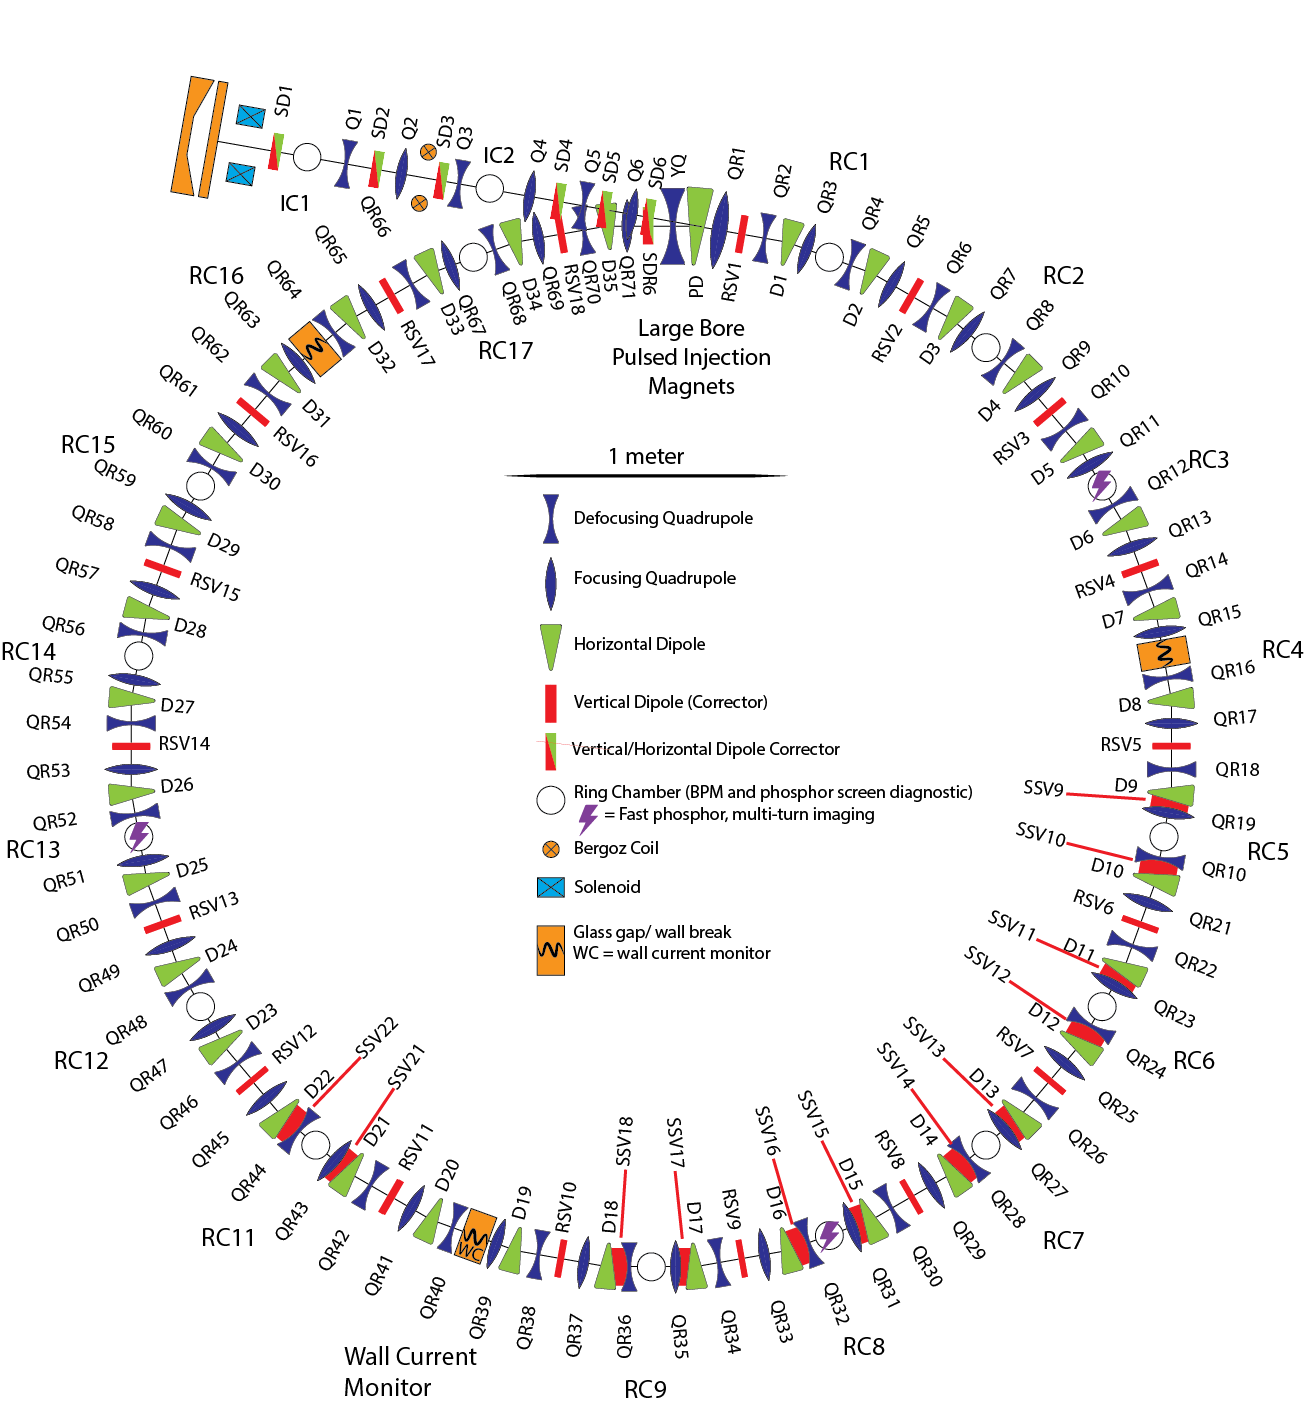
\includegraphics[width=\textwidth]{umer-diagram/full_ring.png}
   \caption{UMER ring, with all magnets labelled.}
   \label{fig:umerring}
\end{figure}

\subsection{Alternative FODO lattice}

\begin{figure}[]
%   \vspace*{-.5\baselineskip}
   \centering
   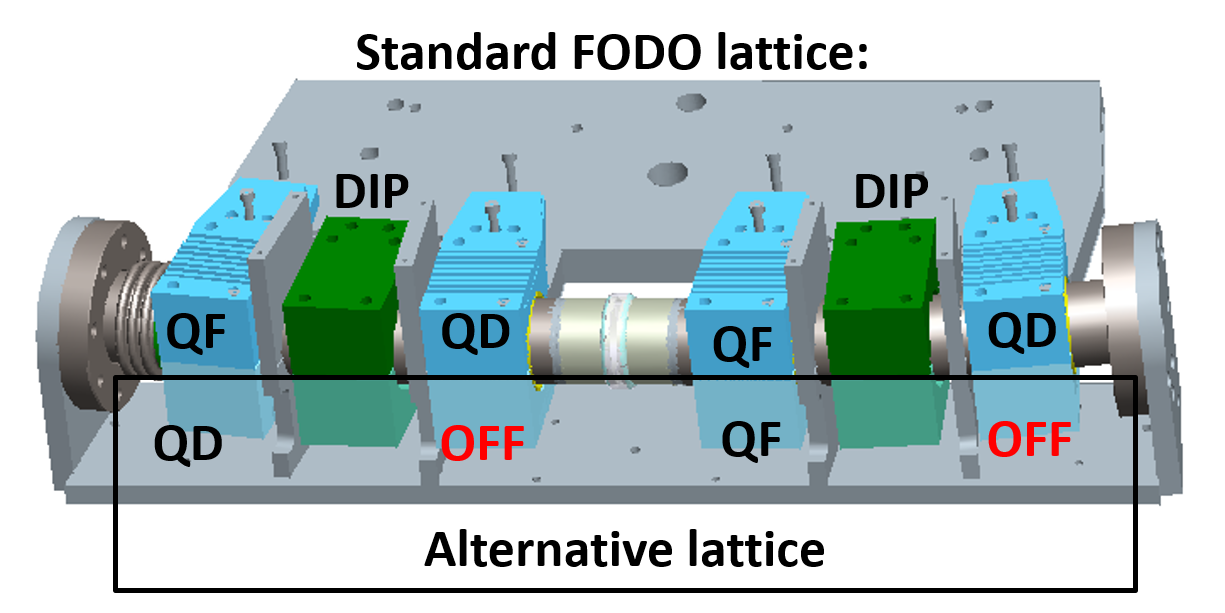
\includegraphics[width=0.7\textwidth]{6.figures/UMER_FODO.png}
   \caption{Two standard UMER FODO cells (blue quadrupoles and green dipoles). In the Alternatice lattice, the crossed quadrupoles are unpowered, leaving a vacancy for octupole elements.}
   \label{fig:FODOcell}
%   \vspace*{-\baselineskip}
\end{figure}

\begin{figure}[]
   \centering
   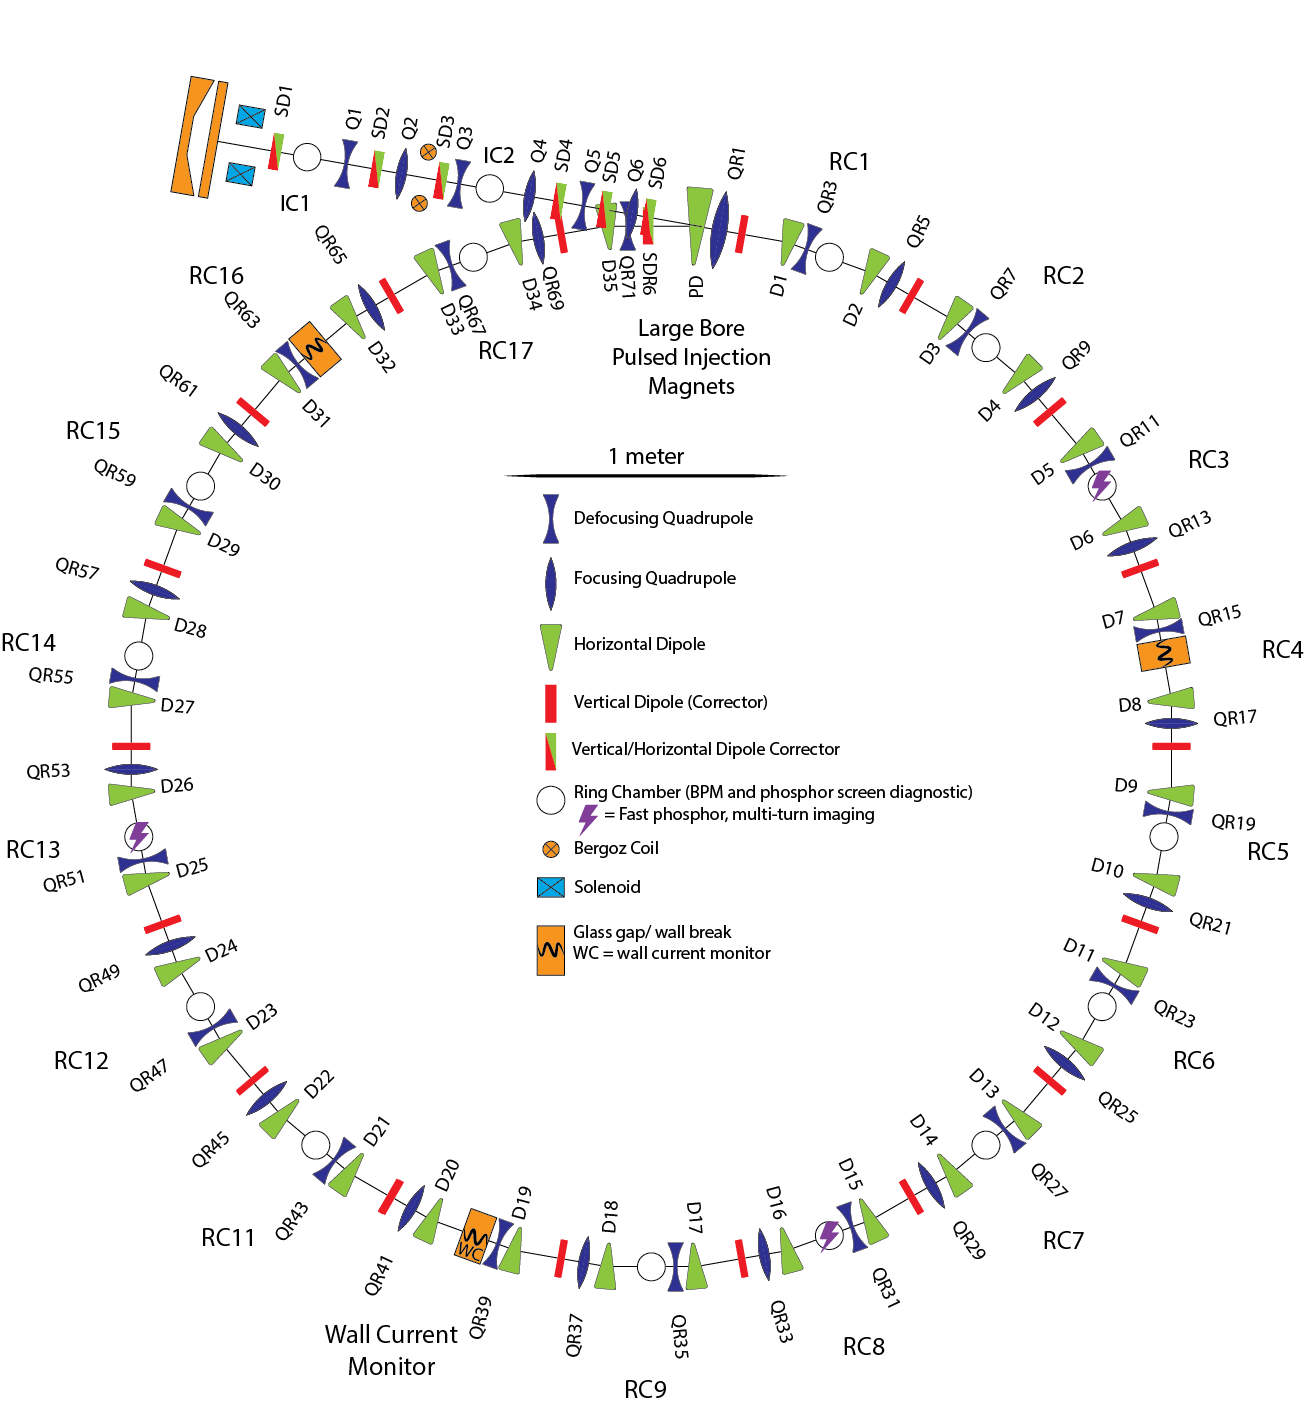
\includegraphics[width=\textwidth]{umer-diagram/altlat_full_ring.png}
   \caption{UMER ring in alternative lattice configuration.}
   \label{fig:altlatring}
\end{figure}

This configuration utilizes a mode of UMER operation known as the “alternative lattice” in which the total number of FODO cells in the ring is halved (by removing half of the quadrupoles).  The two lattices are illustrated in Fig. \ref{fig:FODOcell}. The nominal tune of the ring is also approximately halved, from $\nu \approx 6.7$ to $\approx 3.8$.



\subsection{Octupole Lattices}

%%%%%%%%%%%%%%%%%%%%%%%%%%%%%%%%%%%%%%%%%%%%%%%%%%%%%%%%%%%%%%%%%%%%%%%%%%%%%%%%%%%%%%%%%%%%%%%%%%%%%%%%%%%%%%%%%%%%%%%%%%
%% from AAC14
%%%%%%%%%%%%%%%%%%%%%%%%%%%%%%%%%%%%%%%%%%%%%%%%%%%%%%%%%%%%%%%%%%%%%%%%%%%%%%%%%%%%%%%%%%%%%%%%%%%%%%%%%%%%%%%%%%%%%%%%%%
We will modify the ring to include an octupole channel, while maintaining existing ring element placement for easy conversion between nonlinear and FODO lattice configurations. As shown in Fig. 2b, the planned lattice includes a single channel, occupying ~3% of the ring (or 32 cm, the longest straight section). WARP simulations will determine if this design is sufficient to produce an observable effect on beam halo, or if a longer octupole is necessary. Possible alternate configurations include two octupole channels, a longer channel encompassing one or more dipoles (if dispersive effects allow) or, in the extreme case, a long straight (> 32 cm) pipe section in a modular design that can be temporarily installed for these experiments. All but the latter configuration allow the preservation of the linear FODO lattice by superimposing the octupole lattice over existing quadrupole and dipole circuits. The user will be able to switch between linear and nonlinear operation simply by changing power supply settings.  
Two options exist for octupole magnet design. The first, visualized in Fig. 1, is a quasi-continuous channel composed of multiple short octupoles (~ 4 cm length) with overlapping fields, that “fill-in” the 1⁄〖β(s)〗^3  octupole strength variation. This option allows fine-tuning of the longitudinal strength profile and permits use of existing magnet mounts. The second option is to print the octupole channel as a single, axially extended circuit, which eliminates alignment errors between the components and creates a “frozen-in” longitudinal profile. This reduces the need for additional power supplies but requires redesign of magnet mounts in that section.
The octupole channel occupies only a small fraction of the ring. The remainder of the ring must act as an external lens that simulates continuous transport through the channel. The linear portion of the nonlinear UMER configuration will consist of a reduced-density FODO section and two matching sections bordering the octupole insert. The reduced-density lattice (or “alternative lattice” [5]) is chosen to avoid asymmetries introduced by a pulsed quadrupole at the beam injection. Elegant code calculations identified several lattice solutions to achieve a symmetric beam in the octupole. One solution is pictured in Fig. 2a.  Quadrupole gradients in the matching sections range from 76% to 117% of the typical operating point in the alternative lattice.
%%%%%%%%%%%%%%%%%%%%%%%%%%%%%%%%%%%%%%%%%%%%%%%%%%%%%%%%%%%%%%%%%%%%%%%%%%%%%%%%%%%%%%%%%%%%%%%%%%%%%%%%%%%%%%%%%%%%%%%%%%

\section{Printed Circuit Octupoles}


%%%%%%%%%%%%%%%%%%%%%%%%%%%%%%%%%%%%%%%%%%%%%%%%%%%%%%%%%%%%%%%%%%%%%%%%%%%%%%%%%%%%%%%%%%%%%%%%%%%%%%%%%%%%%%%%%%%%%%%%
% Copy from conf paper
%%%%%%%%%%%%%%%%%%%%%%%%%%%%%%%%%%%%%%%%%%%%%%%%%%%%%%%%%%%%%%%%%%%%%%%%%%%%%%%%%%%%%%%%%%%%%%%%%%%%%%%%%%%%%%%%%%%%%%%%
% \begin{figure}[]
% %   \vspace*{-.5\baselineskip}
   % \centering
   % 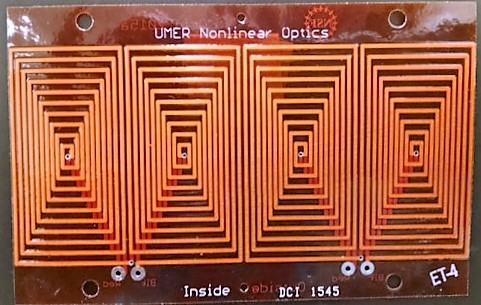
\includegraphics[0.5\textwidth]{3.figures/octupole_PCB}
   % \caption{Half of a UMER printed circuit octupole magnet}
   % \label{fig:octupcb}
% %   \vspace*{-\baselineskip}
% \end{figure}

% \begin{figure}[]
% %   \vspace*{-.5\baselineskip}
   % \centering
   % \includegraphics*[0.5\textwidth]{3.figures/OctupoleFFTreal}
   % \caption{FFT measurement of octupole from rotating coil measurement}
   % \label{fig:octurotcoil}
% %   \vspace*{-\baselineskip}
% \end{figure}


MER utilizes air core printed circuit magnets, pictured in Fig. 1, for focusing and steering. The printed circuits are incredibly cost-effective as well as lightweight and stackable, making any combination of multipoles possible. They can operate in DC or pulsed mode, and are easily tunable with no hysteresis. 
The octupole inserts will be based on the UMER quadrupole design. Outfitting UMER for nonlinear experiments will be a relatively low-cost upgrade.

The first generation of printed circuit octupoles has been produced and initial characterization made. The PC circuits, pictured in Fig \ref{fig:octupcb}, are made in two double-layered halves, which fit inside the standard UMER quadrupole mount. Based on the similarity to existing UMER PC quadrupoles and dipoles, each magnet should easily be able to sustain 2 A DC with the existing mounts and up to 10 A with addition of water cooling. Maxwell 3D calculations show $75 T/m^3/A$ peak fields in the octupole, with the 16-pole as the next significant multipole, against theoretical predicts that the 24-pole is the next highest allowed multipole. \cite{VenturiniThesis}

The magnet has been characterized using an integrated rotating coil measurement. A long coil rotating at 1 Hz sends EMF signal to an oscilloscope. The resulting scope FFT can be seen in Fig. \ref{fig:octurotcoil}. The large dipole contribution is primarily due to the earth’s magnetic field. Sextupole and quadrupole terms are minimized by adjusting the transverse position of the octupole.


\cite{BaumgartnerNAPAC2016}
%%%%%%%%%%%%%%%%%%%%%%%%%%%%%%%%%%%%%%%%%%%%%%%%%%%%%%%%%%%%%%%%%%%%%%%%%%%%%%%%%%%%%%%%%%%%%%%%%%%%%%%%%%%%%%%%%%%%%%%%

\section{Simulation Codes}
\subsection{WARP}
\cite{warp}
%%%%%%%%%%%%%%%%%%%%%%%%%%%%%%%%%%%%%%%%%%%%%%%%%%%%%%%%%%%%%%%%%%%%%%%%%%%%%%%%%%%%%%%%%%%%%%%%%%%%%%%%%%%%%%%%%%%%%%%%

\subsection{Elegant}
\cite{elegant}
%%%%%%%%%%%%%%%%%%%%%%%%%%%%%%%%%%%%%%%%%%%%%%%%%%%%%%%%%%%%%%%%%%%%%%%%%%%%%%%%%%%%%%%%%%%%%%%%%%%%%%%%%%%%%%%%%%%%%%%%

\subsection{VRUMER}
%%%%%%%%%%%%%%%%%%%%%%%%%%%%%%%%%%%%%%%%%%%%%%%%%%%%%%%%%%%%%%%%%%%%%%%%%%%%%%%%%%%%%%%%%%%%%%%%%%%%%%%%%%%%%%%%%%%%%%%%
\section{Simulation Techniques}
\subsection{Frequency Map Analysis}

A standard approach to understanding long term behaviour of single particle dynamics in an accelerator, particularly the effects of nonlinearities and resonances on dynamic aperture, is frequency map analysis (FMA). Originally applied to study of celestial mechanics, the technique has been successfuly applied to accelerator dynamics [\cite{Laskar2003}]. This is a powerful technique for simulation studies, but has also been applied to experimental data as well. 

As applied to UMER lattices, many test particles are launched over a range of possible initial conditions and the orbits tracked over a long path length. I calculate fundamental orbit frequency, splitting the orbit into two halves ($t_o \to t_{mid}$ and $t_{mid} \to t_{final}$) to obtain two frequency values, $\nu_1$ and $\nu_2$. The difference between these values, $\Delta \nu = \nu_1-\nu_2$ is a measure of chaos in the orbit. An orbit with irregular frequency will typically have a large $\Delta \nu$, while $\Delta \nu \to 0$ for regular orbits. 

It can be useful to plot $\Delta \nu $ versus initial conditions, which indicates dynamics aperture. Lines of high $\Delta \nu$ indicate resonance structures, which may or may not contribute to aperture limitation through particle diffusion. Another approach is to plot $\Delta \nu $ versus fundamental frequency, which depicts the "tune footprint," or frequency space inhabited by the beam. Again, high $\Delta \nu$ will align with resonance lines in the tune diagram, allowing easy identification of harmful resonances. 

In accelerators, position data used for frequency calculation is often limited in length. Frequency resolution using Fourier transformation scales as $\frac{1}{N}$ for number of sample points $N$. For higher precision, most algorithms use Numerical Analysis of Fundamental Frequency (NAFF), with a resolution $\propto \frac{1}{N^4}$. 

%todo: describe NAFF



FMA is built-in in many standard accelerator codes, including Elegant. While not included in standard WARP packages, I wrote an FMA module accessed at the Python level. 